\documentclass{patmorin}
\usepackage{amsthm,amsmath,graphicx}
\usepackage{pat}
%\usepackage{coffee4}


\DeclareMathOperator{\asf}{asf}
\DeclareMathOperator{\depth}{depth}
\DeclareMathOperator{\radius}{radius}
\newcommand{\mand}{\mathrm{,\,\,and\,}}
\newcommand{\oand}{\mathrm{,\,\,}}

\title{\MakeUppercase{Good-Average-Stretch Geometric Spanners}}
\author{Vida Dujmovi\'c, Pat Morin, and Michiel Smid}


\begin{document}
\begin{titlepage}
\maketitle
%\cofeAm{0.7}{0.38}{0}{5.5cm}{3.5in}

\begin{abstract}
  We show that, for any set $V$ of $n$ points in $\R^d$, there exists
  a geometric graph with vertex set $V$, $O(n)$ edges, and that has
  average stretch factor $1+ O((\log n/n)^{1/2d})$.
  We also show that, even in $\R^2$, there exists point sets for which
  any graph with a linear number of edges has average stretch factor
  at least $1+\Omega(1/\sqrt{n})$.
\end{abstract}

\end{titlepage}

\section{Introduction}

The \emph{average stretch factor} of a geometric graph, $G$, with vertex
set $V(G)\subset \R^d$ and edge set $E(G)$ is
\[
    \asf(G) = \binom{|V(G)|}{2}^{-1}\sum_{\{u,w\}\in\binom{V(G)}{2}}\frac{\|uw\|_G}{\|uw\|} \eqlabel{asf}
\]
where $\|uw\|$ denotes the Euclidean distance between $u$ and $w$
and $\|uw\|_G$ denotes the shortest Euclidean path from $u$ to $w$
that uses only edges of $G$.

In this paper we show that, for any constant dimension, $d$, and any
finite set $V\subset \R^d$, there exists a geometric graph $G=(V,E)$
having $|E|=O(n)$ edges and such that $\asf(G)=1+o_n(1)$.

\section{The Construction}

The construction of a good average stretch factor graph, $G=(V,E)$,
makes use of a clustering of the points of $V$ into $O(n/k)$ clusters of
size at most $k$ that we call a $k$-partition.  In the next subsection,
we define $k$-partitions and show how to compute them.  In the following
subsection we show how to construct the graph $G$.

\subsection{$k$-Partitions}

We make use of the following construct:  A \emph{$k$-partition} of a
set $V$ of $n$ points in $\R^d$ consists of a set, $D$, of balls and an
assignment $f:V\to D$ such that
\begin{enumerate}
  \item $|D|\in O(n/k)$;
  \item for each $u\in V$, $u\in f(u)$ (i.e., $u$ is a assigned to a
    ball that contains $u$);
  \item for each $\Delta\in D$, $|\{u\in V: f(u)=\Delta\}|\le k$ (i.e.,
   at most $k$ points are assigned to each ball);
  \item for every $r> 0$, $c\ge 2$, and $p\in\R^2$, the number of balls
   in $D$ whose radius is in the range $[r,2r)$ and that contain $p$
   is $O(1)$; and
  \item for every $r\ge 0$, $c>1$ and every ball, $B$, of radius $r$, the set
    \[  \{ u\in V : u\in B\oand \Delta\in D\oand \radius(\Delta)\ge\radius(B)/c\oand f(u)=\Delta\mand \Delta\cap B\neq\emptyset\} \]
   has cardinality $O(k\log c)$.
\end{enumerate}

Note that, aside from Properties~4 and 5, there is very little structure to
the balls in $D$. In particular, balls in $D$ may overlap and may even
contain each other.

\begin{lem}
  For any set $V$ of $n$ points, a $k$-partition of $V$ exists and can
  be found in $O(n\log n)$ time.
\end{lem}

\begin{proof}
  We construct a $k$-partition using the binary \emph{fair-split
  tree}, $T=T(V)$, which is defined recursively as follows
  \cite{callahan.kosaraju:decomposition}: If $V$ consists of a single
  point, $u$, then $T$ contains a single node corresponding to $u$.
  Otherwise, consider the minimal axis-aligned bounding box, $B(V)$,
  that contains $V$.  The root of $T$ corresponds to $B(V)$ and this
  box is split into two boxes $B_1(V)$ and $B_2(V)$ by cutting $B(V)$
  with a hyperplane in the middle of its longest side.  The left and
  right subtrees of the root are defined recursively by constructing
  fair-split trees for $B_1(V)\cap V$ and $B_2(V)\cap V$. See \figref{fst}.

  \begin{figure}
    \begin{center}
      \includegraphics{whole-thing}
    \end{center}
    \caption{A fair split tree for $V$ repeatedly by splits the bounding
      box $B(V)$ in the middle of its longest side.}
    \figlabel{fst}
  \end{figure}

  \paragraph{The $k$-Partition.}
  For each node, $u$, of $T$ there is a naturally defined subset
  $V(u)\subseteq V$ of points associated with $u$ as well as a bounding
  box $B(u)=B(V(u))$.  Since $T$ is a binary tree with $2n+1$ nodes, it
  has a set of $t-1$ edges whose removal partitions the vertices of $T$
  into $t\in O(n/k)$ maximally-connected components $C_1,\ldots,C_t$,
  each having at most $k$ vertices.

  For each $i\in\{1,\ldots,t\}$, let $u_i$ denote the root of the
  subtree $C_i$.  To obtain the balls, $\Delta_1,\ldots,\Delta_t$, of
  the $k$-partition we take, for each $i\in\{1,\ldots,t\}$ the smallest
  ball, $\Delta_i$ that contains $B(u_i)$.  For the mapping $f$, we
  map the point associated with each leaf, $w$, of $T$ to the unique
  ball $\Delta_i$, where $C_i$ contains $w$.  (Note that some balls,
  $\Delta_i$, may have no points mapped to them if $C_i$ contains no
  leaves of $T$; see \figref{fst-2}.)

  \begin{figure}
    \begin{center}
      \includegraphics{whole-thing2}
    \end{center}
    \caption{The fair split tree is partitioned into subtrees of size
    $k$ (${}=3$) by removing $O(n/k)$ edges.  The root, $u_i$, of each subtree
    defines a ball, $\Delta_i$, in the $k$-partition. (The ball $\Delta_1$
    is omitted from this figure.)}
    \figlabel{fst-2}
  \end{figure}


  The fair-split tree, $T$, and the boxes, $B(u)$, associated
  with each node, $u$, of $T$ can be computed in $O(n\log n)$ time
  \cite{callahan.kosaraju:decomposition}.  The partition of the vertices
  of $T$ into components $C_1,\ldots,C_t$ can easily be done in $O(n\log
  n)$ time by repeatedly finding an edge of a component of size $k'>k$
  that partitions that component into two pieces each of size at most
  $\lceil 2k'/3\rceil$.  Thus, the construction of $D$ and $f$ can be
  accomplished in $O(n\log n)$ time.

  The set of balls $D=\{\Delta_1,\ldots,\Delta_t\}$ and the mapping
  $f:V\to D$ described in the preceding paragraphs clearly satisfy
  Properties~1--3 in the definition of a $k$-partition.  What remains
  is to show that they also satisfy Properties~4 and 5. For a node
  $u$ in $T$, let $L(u)$ denote the length of the longest side of
  $B(u)$.  We make use of the following result on fair split trees
  \cite[Lemma~9.4.3]{narasimhan.smid:geometric}:

  \begin{lem}\lemlabel{box-packing}
     Let $C$ be a box whose longest side has length $\ell$ and let
     $\alpha >0$ be any positive real number.  Let $w_1,\ldots,w_s$
     be some nodes of a fair-split tree, $T$, such that
     \begin{enumerate}
       %\item $w_i$ is not the root of $T$, for all $i\in\{1,\ldots,s\}$;
       \item the sets $V(w_i)$ are disjoint, for all $i\in\{1,\ldots,s\}$;
       \item $L(w_i)\ge \ell/\alpha$, for all
          $i\in\{1,\ldots,s\}$;\footnote{The original lemma
          \cite[Lemma~9.4.3]{narasimhan.smid:geometric} is slightly
          stronger in that it only requires that $L(w_i')\ge \ell/\alpha$,
          where $w_i'$ is the parent of $w_i$.} and
       \item $B(w_i)$ intersects $C$, for all $i\in\{1,\ldots,s\}$.
     \end{enumerate}
     Then $s\le (2\alpha + 2)^d$.
  \end{lem}
  %Note that the first condition of \lemref{box-packing} is equivalent
  %to the statement that no $u_i$ is an ancestor of $u_j$ for any
  %$\{i,j\}\subseteq\{1,\ldots,k\}$, which also implies that the interiors of
  %$B(u_i)$ and $B(u_j)$ are disjoint.

  \paragraph{Property 4.}
  To prove that the balls in $D$ satisfy Property~4, let
  $\{\Delta_{i_1},\ldots,\Delta_{i_q}\}\subseteq D$ be the subset of
  balls in $D$ having radii in the interval $[r,2r)$ and that all contain
  some common point, $p\in\R^d$.   Then each such ball, $\Delta_{i_j}$
  corresponds to a node $u_{i_j}$ of $T$ such that
  \begin{equation}
        \frac{r}{\sqrt{d}} \le L(u_{i_j}) \le 4r \enspace . \eqlabel{bounds}
  \end{equation}
  Therefore, each box $B(u_{i_j})$ intersects a ball of radius $2r$
  centered at $p$.  (Indeed, the center of $B(u_{i_j})$ is contained in
  this ball.)  Therefore, each box $B(u_{i_j})$ intersects a box, $C$, of
  side-length $4r$ centered at $p$.  

  We are almost ready to apply \lemref{box-packing} to
  $C$---whose side length is $\ell = 4r$---and the vertex set
  $w_1,\ldots,w_q=u_{i_1},\ldots,u_{i_q}$. For each $j\in\{1,\ldots,q\}$,
  $B(u_{i_j})$ intersects $C$, so Condition~3 of \lemref{box-packing}
  is satisfied.  Furthermore, \eqref{bounds} states that $L(u_{i_j})\ge
  r/\sqrt{d} = \ell/(4\sqrt{d})$, so Condition~2 of \lemref{box-packing}
  is satisfied with $\alpha=4\sqrt{d}$.  Unfortunately, there is still
  a little more work to do since the nodes $u_{i_1},\ldots,u_{i_t}$
  do not necessarily satisfy Condition~1 of \lemref{box-packing}.

  To proceed, we partition $u_{i_1},\ldots,u_{i_q}$ into a small number of
  subsets, each of which satisfies Condition~1 of \lemref{box-packing}.
  Observe that Condition~1 of \lemref{box-packing} is equivalent
  to the statement that no $w_i$ is an ancestor of $w_j$ for any
  $\{i,j\}\subseteq\{1,\ldots,s\}$.  A key observation is that, if $u$
  is an ancestor of $w$ in a fair-split tree, $T$, and the difference
  in depth between $u$ and $w$ is $d$, then
  \[
      L(u) \ge 2L(w) \enspace .
  \]
  This, and \eqref{bounds}, implies that, if $u_{i_j}$ is an ancestor
  of $u_{i_{j'}}$ then
  \[
     \depth(u_{i_{j'}})-\depth(u_{i_{j}}) \le d\log(4\sqrt{d}) \enspace .
  \]
  Thus, we can partition $u_{i_1},\ldots,u_{i_q}$ into $z=\lceil
  d\log(4\sqrt{d})\rceil$ subsets, $S_0,\ldots,S_{z-1}$, each of which
  satisfies Condition~1 of \lemref{box-packing}, by assigning $u_{i_j}$
  to the subset $S_{\depth(u_{i_j})\bmod z}$.  

  Now, \lemref{box-packing} implies that, for each $i\in\{0,\ldots,z-1\}$, 
  \[
     |S_i|\le (8\sqrt{d}+2)^d
  \]
  so that
  \[
     q = \sum_{i=0}^{z-1}|S_i|\le (8\sqrt{d}+2)^dz = (8\sqrt{d}+2)^d\lceil d\log(4\sqrt{d})\rceil  \in O(1) \enspace .
  \]
  Thus, for any point $p\in\R^d$, the set of balls in $D$ whose radius
  is in the interval $[r,2r)$ and that contain $p$ has size $O(1)$.
  Therefore the balls in $D=\Delta_1,\ldots,\Delta_t$ satisfy Property~4
  in the definition of a $k$-partition.

  \paragraph{Property 5.}
  TODO: Prove this.
\end{proof}

\subsection{The Graph $G$}

With the availability of $k$-partitions, we are now ready to prove
construct a graph $G$ with low average stretch.  In the following
construction, positive valued variables $c,k\in\omega_n(1)$ and
$\epsilon\in o_n(1)$ are used without being specified.  Values of these
variables that optimize the average spanning ratio of $G$ will be given
in the proof that $\asf(G)\in 1+o_n(1)$.

We begin with a $k$-partition $(\{\Delta_1,\ldots,\Delta_{n'}\},f)$
of $V$, and we use the convention that $\Delta_1,\ldots,\Delta_{n'}$
are ordered by decreasing size.  For each $i\in \{1,\ldots,n'\}$,
let $V_i=\{u\in V : f(u)=\Delta_i\}$; that is, $V_i$ is the set of
points assigned to the ball $\Delta_i$.  For each set $V_i$, we choose a
representative vertex, $u_i$, and add edges joining $u_i$ to each other
vertex in $V_i$ (see \figref{overview}). Let $N=\{u_1,\ldots,u_{n'}\}$
denote the set of representative vertices and recall that $|N|=n'\in
O(n/k)$.

\begin{figure}
  \begin{center} 
    \includegraphics{overview}
  \end{center} 
  \caption{Using a $k$-partition, $G$ contains $O(n/k)$ stars whose
    centers are interconnected by a $(1+1/k^{1/(d-1)})$-spanner}
  \figlabel{overview}
\end{figure}

Next, we add two spanner constructions to $G$.  The first is a
$(1+1/k^{1/(d-1)})$-spanner of $N$ and the second is a $2$-spanner
of $V$.  The first construction adds $O(k|N|)=O(n)$ edges to $G$
\cite[Section~5.5]{narasimhan.smid:geometric}, while the second adds
$O(n)$ edges \cite{x,ys,ss}.  With the addition of these extra edges we
have, for any $u,w\in V$
\[
   \frac{\|uw\|_G}{\|uw\|} \le \begin{cases}
         1+1/k^{1/(d-1)} & \text{if $u,w\in N$} \\
         2 & \text{in any case.}
       \end{cases}
\]

Let $r_i$ denote the radius of $\Delta_i$ and let $D_i$ be a ball centered
at the center of $\Delta_i$ and having radius $cr_i$.  Points of $V$
that are in $D_i\setminus \Delta_i$ can be problematic for $V_i$; there
is no guarantee that such points have a $1+o(1)$ spanning path to the
points in $V_i$.  The final step in the spanner construction attempts
to deal with most of these problematic points.

For each $i\in\{1,\ldots,n'\}$, we find a ball, $E_i$, of radius $r_i/c$,
that intersects $D_i$, and that contains the maximum number of points
of $V$.  (Note that this may include points of $V$ in $V_i$ or outside
of $D_i$.)  We then add edges joining each of the points in $V_i$ to
some point, $w_i$, in $E_i$.  See \figref{hitter}.

The point $w_i\in E_i$ is carefully chosen as follows: For each point
$w\in V$, let $i(w)\in \{1,\ldots,n'\}$ denote the smallest index such
that $w\in E_{i(w)}$ and $|E_{i(w)}\cap V| \ge \epsilon n$; if no such
index exists, let $i(w)=\infty$.  The point $w_i\in E_i$ is selected
to be any of the points in $E_i$ that minimizes $i(w)$.  This concludes
the description of the graph, $G$.  The following theorem shows that $G$
is a good-average-stretch spanner.

\begin{figure}
  \begin{center}
    \includegraphics{hitter}
  \end{center}
  \caption{The ball $E_i$ captures as many points of $V$ as possible
   while still having center in $D_i$.}
  \figlabel{hitter}
\end{figure}

\begin{thm}\thmlabel{upper-bound}
  For every constant dimension, $d$, and every set, $V$, of
  $n<\infty$ points in $\R^d$, the graph $G=(V,E)$ described above
  has $O(n)$ edges and $\asf(G)=1+o_n(1)$.
  % there exists a geometric graph $G$ with
  % $V(G)=V$, $|E(G)|\in O(n)$ and $\asf(G)=1+o_n(1)$. 
  % More precisely, $\asf(G)=1+O((\log n/n)^{1/2d})$.
\end{thm}

\begin{proof}
  That $G$ has $O(n)$ edges follows immediately from its definition.

  To determine the average stretch factor of $G$, there are four types
  of pairs of points, $u\in V_i$, $w\in V_j$, $j\ge i$, to consider:
  \begin{enumerate}
    \item pairs that are both from the same set; i.e., where $i=j$;
    \item pairs for which $w$ is outside of $D_i$;
    \item pairs for which $w$ is contained in $E_i\cap D$; and
    \item pairs for which $w$ is contained in $D_i\setminus E_i$.
  \end{enumerate}
  In the next few section we consider each of these pairs in turn.
  Our strategy is to study the $\binom{n}{2}$ terms that define $\asf(G)$
  in \eqref{asf}.  We will show that $o(n^2)$ of these terms are at most
  2 while the remaining terms are at most $1+o_n(1)$.  Thus,
  \[
     \asf(G)\le \binom{n}{2}^{-1}\left(2\cdot o(n^2)
                                       +\binom{n}{2}(1+o_n(1))\right)
     = 1+o_n(1) \enspace .
  \]

  \paragraph{Type~1 Pairs.}
  For each Type~1 pair $u,w\in V_i$, $\|uw\|_G/\|uw\|\le 2$ and each set
  $V_i$ contributes at most $\binom{k}{2}$ Type~1 terms to \eqref{asf},
  so the total contribution of Type~1 pairs to the sum in \eqref{asf} is at most
  \[
    \binom{k}{2}\cdot 2 \cdot O(n/k) \in O(nk)
      \enspace .
  \]

  \paragraph{Type~2 Pairs.}
  For Type~2 pair $u\in V_i$, $w\in V\setminus D_i$, there is a path
  from $u$ to $u_i$ and then onto $u_j$ and finally to $w$ whose length
  is at most
  \[
     r_i + \|u_iu_j\|_G + r_j
      \le (1+1/k^{1/(d-1)})(\|uw\| + 8r_i) \enspace .
  \]
  Furthermore, $\|uw\|\ge (c-1)r_i$ since $w$ is outside of $D_i$.
  Therefore,
  \[
    \frac{\|uw\|_G}{\|uw\|}\le (1+1/k^{1/(d-1)})(1+O(1/c)) 
       \in 1+O(1/k^{1/(d-1)}+1/c) \enspace .
  \]

  \paragraph{Type~3 Pairs.}
  The number of Type~3 pairs is no more than $k\sum_{i=1}^{n'}|V\cap
  D_i\setminus E_i|$, so the total contribution of Type~3 pairs to 
  the sum in \eqref{asf} is at most
  \[
      2\cdot\left(k\sum_{i=1}^{n'} |V\cap D_i\setminus E_i|\right) \enspace .
  \]
  We intend to prove, by contradiction, that the preceding quantity
  is $o(n^2)$.  Suppose, for the sake of contradiction, that this is
  not the case and that
  \begin{equation}
    \delta n^2/k \le \sum_{i=1}^{n'} |V\cap D_i\setminus E_i| 
         \enspace . \eqlabel{kicker}
  \end{equation}
  Each term on the right hand side of \eqref{kicker} is at most $n$
  and there are at most $\alpha n/k$ terms, for some constant $\alpha
  >0$.  We say that a term on the right hand side of \eqref{kicker} is
  \emph{small} if it is less than $\delta n/2\alpha$ and \emph{large}
  otherwise.  The sum of the small terms is at most $\delta n^2/2k$
  and therefore the sum of the large terms is at least $\delta n^2/2k$.
  Let $I$ be the index set of these large terms.  Then
  \[
    \sum_{i\in I} |V\cap D_i\setminus E_i| \ge \frac{\delta n^2}{2k} \enspace .
  \]
  By the pigeonhole principle, there must exist some point $w^*\in V$
  such that there are at least $\delta n/2k$ indices $i\in I$ such
  that $w^*\in V\cap D_i\setminus E_i$.  To summarize: There exists a
  point $w^*\in V$ and indices $i_1,\ldots,i_\ell$ such that:
  \begin{enumerate}
     \item $w^*\in V\cap D_{i_j}\setminus E_{i_j}$, for all
        $j\in\{1,\ldots,\ell\}$;
     \item $|V\cap D_{i_j}\setminus E_{i_j}|\in \Omega(\delta n)$,
       for all $j\in\{1,\ldots,\ell\}$; and
     \item $\ell\in\Omega(\delta n/k)$.
  \end{enumerate}

  Suppose, without loss of generality, that the smallest ball
  in $D_{i_1},\ldots,D_{i_\ell}$ has unit radius.  Partition
  $i_1\ldots,i_\ell$ into groups $G_0,G_1,\ldots$ such that $G_t$
  contains all indices $i_j$ such that $D_{i_j}$ has radius in the
  interval $[2^t,2^{t+1})$.  We claim that each such group, $G_t$, has
  size $O(c^d)$.  To see why this is so, observe that, for each group
  $G_t$, there exists a point $w^*\in V$ that is contained in $|G_t|$
  balls $D_{i}$ where $i\in G_t$.  $D_{i}$ has radius at most $c2^{t+1}$.
  This means that the set of balls
  \[
     \{ \Delta_i : i\in G_t\}
  \]
  is contained in a ball, centered at $w^*$, of radius at most
  $(c+1)2^{t+1}$.  Since each ball in this set has radius in
  $[2^t,2^{t+1})$, a simple packing argument that uses Property~4 of
  $k$-partitions implies that the size of $G_t$ is $O(c^d)$.

  Thus far, we have shown that each group, $G_t$, has size $O(c^d)$
  and the total size of all groups is $\ell\in\Omega(\delta n/k)$.
  Therefore, there must be at least $\Omega(\delta n/(kc^d))$ groups.
  In particular, we can find $h\in\Omega(\delta n/(kc^d\log c))$ groups,
  $G_{t_1},\ldots,G_{t_h}$, such that $t_{i+1} \ge t_{i}+2\log c+2$ for
  each $i\in\{1,\ldots,h-1\}$.  By selecting a representative element from
  each of these groups, we obtain a sequence of indices $i_1,\ldots,i_h$
  such that the radius of $\Delta_{i_{j+1}}$ is at least $4c^d$ times
  the radius of $\Delta_{i_j}$ for each $j\in\{1,\ldots,h-1\}$.

  By choice, $D_{i_1}$ contains at least $ a \delta n$ elements of
  $V$, for some constant $ a  >0$.  Also by choice, $D_{i_2}\setminus
  E_{i_2}$ contains at least $ a \delta n$ elements of $V$.
  Both $D_{i_1}$ and $D_{i_2}$ contain the point $w^*$.  We claim
  that $E_{i_2}$ contains at least $ a \delta n$ elements of $V$
  as well since there exists a ball, $E_{i_2}'$, centered at $w^*$,
  of radius $r_{i_2}/c > 4cr_{i_1}$, that contains $D_{i_1}$ and
  therefore contains all the (at least $ a  n$) points in $D_{i_1}$
  (see \figref{containment}).  The ball $E_{i_2}$ was chosen to contain
  as many elements of $V$ as possible, so it contains at least as many
  elements as $E_{i_2}'$.  Therefore, $D_{i_2}\cup E_{i_2}$ contains at
  least $2 a  \delta n$ points of $V$.

  \begin{figure}
     \begin{center}
       \includegraphics{containment}
     \end{center}
     \caption{$D_{i_2}\cup E_{i_2}$ contains at least $2 a  n$ 
              points of $V$.}
     \figlabel{containment}
   \end{figure}

  We can now argue similarly to show that $E_{i_3}$ contains at
  least $2 a \delta n$ points of $V$ so $D_{i_3}\cup E_{i_3}$
  contains at least $3 a \delta n$ points of $V$.  In general,
  this argument shows that $D_{i_h}\cup E_{i_h}$ contains at least
  $h a \delta n$ points of $V$.  But this yields a contradiction for
  $h> 1/ a \delta$, since $V$ contains only $n$ points.  This means
  that our choice of $\delta$, $c$, and $k$ must satisfy
  \[
       h\in\Omega\left(\frac{\delta n}{kc^d\log c}\right) \ge
          \frac{1}{ a  \delta}
  \]
  which is satisfied by any choice of $\delta$, $c$, and $k$ such that
  \[
       \frac{\delta^2 n}{kc^d\log c} \ge \frac{1}{a}
  \]
  for some sufficiently large constant $C$.  In particular, the value
  \[
       \delta \ge \frac{1}{a}\sqrt{\frac{kc^d\log c}{n}}
  \]
  works.
  So the total contribution of Type~3 pairs to the sum in \eqref{asf}
  is at most
  \[
    2k\delta n^2 \in O(k^{3/2}n^{3/2}c^{d/2}\log c) \enspace .
  \]

  \paragraph{Type~4 Pairs.}  
  We say that a Type~4 pair of points $u\in V_i$, $w\in E_i$ is
  \emph{bad} if
  \[
      \|uw_i\|+2\|w_iw\| \ge (1+\alpha/c)\|uw\| \enspace ,
  \]
  and otherwise the pair is \emph{good}.
  For any good pair $(u,w)$,
  \[
    \frac{\|uw\|_G}{\|uw\|} = 1+O(1/c) \enspace ,
  \]
  so we can focus our effort on upper-bounding the number of bad pairs.
  The remainder of this proof is a proof by contradiction that will
  assume, for the sake of contradiction, that the number of bad Type~4
  pairs is at least $\epsilon n^2$.

  Let $b_i$ denote the number of number of bad pairs $(u,w)$ with
  $u\in V_i$ and $w\in E_i$.  Then, by assumption,
  \[
    \sum_{i=1}^{n'} b_i \ge \epsilon n^2 \enspace .
  \]
  Applying the same reasoning used to study Type~3 pairs, we can find a
  point $w^*\in V$ and a set of indices $i_1,\ldots,i_{\ell}$ such that
  \begin{enumerate}
    \item $w^*\in E_{i_j}$, for all $j\in\{1,\ldots,\ell\}$;
    \item $b_{i_j} \in \Omega(\epsilon kn)$, for all $j\in\{1,\ldots,\ell\}$;
    %\item $|E_{i_j}\cap V|\in \Omega(\epsilon n)$, for all 
    %    $j\in\{1,\ldots,\ell\}$; and 
    \item $\ell\in \Omega(\epsilon n/k)$.
  \end{enumerate}

  Assume that the indices $i_1,\ldots,i_\ell$ are ordered so that
  $r_{i_j}\le r_{i_{j+1}}$ for all $j\in\{1,\ldots,\ell-1\}$.  Consider
  the sequences of balls $E'_{i_1},\ldots,E'_{i_\ell}$, where each
  $E'_{i_j}$ is a disk of radius $2r_{i_j}/c$ centered at $w^*$. Recall
  that the radius of $E_{i_j}$ is $r_{i_j}/c$, so that $E'_{i_j}\supset
  E_{i_j}$ and, in particular, $|E'_{i_j}\cap V|\ge |E_{i_j}\cap V|$,
  for each $j\in\{1,\ldots,\ell\}$.

  Fix some positive integer $C\in O(1)$ and $t$ to be specified later.
  For each $j\in\{2,\ldots,\ell\}$, let $n_{i_j}=|E'_{i_j}\cap V\setminus
  E'_{i_{j-1}}|$. We have that $\sum_{i=2}^{\ell} n_{i_j} \le n$ and
  $\ell \in\Omega(\epsilon n/k)$.  Using these two bounds, a simple
  averaging argument is sufficient to show that there must exist an
  index $i\in\{2,\ldots,\ell-t-C\}$ such that
  \begin{equation}
     \sum_{j=i}^{i+t+C} n_{i_j}
        = |V\cap E'_{i_{i+t+C}}\setminus \E'_{i_{i}}| 
          \in O((t+C)k/\epsilon) \enspace . \eqlabel{sparse}
  \end{equation}

  Next we observe that the sequence of radii $r_{i_1},\ldots,r_{i_\ell}$
  is exponentially increasing.  More precisely, by Property~4 of
  $k$-partitions\footnote{FIXME: Property 4 needs to be extended a little
  bit.}, there exists an integer constant $\mu$ such that $r_{i_{j+\mu}}
  \ge 2r_{i_j}$ for all $j\in\{1,\ldots,\ell-\mu\}$.  This property,
  and the careful choice of $w_i$'s implies the following claim, whose
  proof is deferred until later.
  \begin{clm}\clmlabel{zuper}
    For every $j\in\{1,\ldots,t\}$, every $u\in V_{i_{i+j}}$, and
    every $w\in E_{i_i}\cap V$, $G$ contains a path of length at most
    $\|uw\|+O(r_{i_i})$.
  \end{clm}

  Let $E$ denote the disk centered at $w^*$ and having radius $cr_{i_i}$.
  Note that any point $u\not\in E$ is at distance at least $(c-1)r_{i_i}$
  from any point $w\in E_{i_i}$.  Therefore, by \clmref{zuper}, for any
  $j\in\{1,\ldots,t\}$ and any $u\in V_{i_{i+j}}\setminus E$,
  \[  
     \frac{\|uw\|_G}{\|uw\|} = 1+O(1/c) \enspace . 
  \]
  In other words, by choosing an appropriate constant $\alpha$ in the
  definition of bad pairs, $u$ can not form a bad pair with a point
  $w\in E_{i_i}$ unless $u$ is contained in $E$.  Consider the disks
  $\Delta_{i_{i+\lceil\mu\log c\rceil}},\ldots,\Delta_{i_{i+t}}$; each
  of which has radius at least $cr_{i_i}$.  By Property~5 of $k$-partitions,
  \[
    \left|\bigcup_{j=\lceil\mu\log c\rceil}^t V_{i_{i+j}}\cap E\right|
      \in O(k)
  \]
  Combining this with \eqref{sparse}, we find that the total number
  of bad pairs of the form $u\in V_{i_{i+j}}$, $w\in E_{i_{i+j}}$,
  and $j\in\{\lceil\mu\log c\rceil,\ldots,t\}$ is upper bounded by
  \begin{equation}
     \sum_{j=\lceil\mu\log c\rceil}^t b_{i_{i+j}} 
        \in O((t+C)k^2/\epsilon) \enspace . \eqlabel{ub-4}
  \end{equation}
  On the other hand, the indices $i_1,\ldots,i_\ell$ are chosen
  so that $b_{i_j}\in\Omega(\epsilon kn)$, for \emph{every}
  $j\in\{1,\ldots,\ell\}$.  Therefore
  \begin{equation}
    \sum_{j=\lceil\mu\log c\rceil}^t b_{i_{i+j}} 
        \in \Omega((t-\lceil\mu\log c\rceil)\epsilon kn) \enspace .
        \eqlabel{lb-4}
  \end{equation}
 
  Equating the right hand sides of \eqref{ub-4} and \eqref{lb-4}, we
  obtain a contradiction when $t>2C$, $t>2\lceil\mu\log c\rceil$, and
  \[
      \epsilon = D\sqrt{k/n}
  \] 
  for a sufficiently large constant $D$.
  Thus, the total number of bad Type~4 pairs is at most
  \[
    \epsilon n^2 \in O(n^{3/2}k^{1/2}) \enspace .
  \]

  All that remains in handling Type~4 pairs is to prove \clmref{zuper}.

  \begin{proof}[Proof of \clmref{zuper}]
  Let $u$ by any point $V_{i_{i+j}}$, for any $j\in\{1,\ldots,t\}$.
  It is sufficient to prove that $\|w^*w_{i_{i+j}}\|\in O(r_{i_i})$.
  If $w_{i_{i+j}}=w^*$, then we are done, so assume $w_{i_{i+j}}\neq
  w^*$.  Since $w^*\in E_{i_{i+j}}$ but was not chosen to act as
  $w_{i_{i+j}}$, there must exist some index $i'$ such that $E_{i'}\cap
  E_{i_{i+j}}\neq\emptyset$, $|E_{i'}\cap V|\ge\epsilon n$, $r_{i'}\le
  r_{i_i}$, and $w_{i_{i+j}}\in E_{i'}$.

  There are two cases to consider:
  If $E_{i_i}$ intersects $E_{i'}$, then 
  \[
     \|w^*w'\|\le r_{i_i} + 2r_{i'} \le 3r_{i_i} \in O(r_{i_i}) \enspace ,
  \]
  and we are done.  On the other hand, if $E_{i'}$ and $E_{i_i}$
  are disjoint, then all the points in $E_{i'}$ are contained in
  $E_{i+t+2\mu}$.  Then
  \[
      |V\cap E_{i+t+2\mu}\setminus E_i| \ge |V\cap\E_{i'}| \ge \epsilon n \enspace .
  \]
  But, by definition, 
  \[
      |V\cap E_{i+t+2\mu}\setminus E_i| \in O(tk/\epsilon) \enspace .
  \]
  This yields a contradiction when $t<D \epsilon^2 n/k$, for a
  sufficiently small constant $D>0$.
  \end{proof}


  \paragraph{Finishing Up.}
  We can now pull everything together.
  \begin{enumerate}
    \item The number of Type~1 pairs is at most $O(kn)$.
    \item For each Type~2 pair, $(u,w)$, 
    \[
      \frac{\|uw\|_G}{\|uw\|}\le 1+ O(1/k^{1/(d-1)}+1/c) \enspace .
    \]
    \item The number of Type~3 pairs is at most
      $O(k^{3/2}n^{3/2}c^{d/2}\log c)$.
    \item For each good Type~4 pair, $(u,w)$, 
    \[
      \frac{\|uw\|_G}{\|uw\|}\le 1+ O(1/c) \enspace .
    \]
    \item The number of bad Type~4 pairs is at most 
       $O(k^{1/2}n^{3/2})$.
  \end{enumerate}
  Putting all four types of pairs together, we obtain
  \[
     \asf(G) = 1 + O\left(1/k^{1/(d-1)} + 1/c 
       + \binom{n}{2}^{-1}\left(kn+k^{3/2}n^{3/2}c^d\log c+k^{1/2}n^{3/2}\right)\right) \enspace .
  \]
  Taking $k=(n/\log n)^{(d-1)/x}$ and $c=(n/\log n)^{1/x}$
  \ldots 
\end{proof}



\section{Lower Bounds}

\begin{thm}\thmlabel{lower-bound}
  For every positive integer $n$, there exists a point set, $V$, of $n$
  points in $\R^2$, such that every geometric graph, $G$, with vertex
  set $V$ and having $O(n)$ edges has $\asf(G)\ge 1 + \Omega(1/\sqrt{n})$.
\end{thm}

\begin{proof}
  For simplicity, we assume $n$ is even.  The point set, $V$, has
  its points evenly distributed on two opposite sides of a square.
  The point set $V=A\cup B$, where
  \[  
      A = \{(1,i): 1\in\{1,\ldots,n/2\}\} 
  \]
  and
  \[  
      B = \{(n/2,i): 1\in\{1,\ldots,n/2\}\} 
  \]
  is an example (see \figref{lower-bound}.a).

  \begin{figure}
    \begin{center}
      \begin{tabular}{c@{\hspace{2cm}}c}
      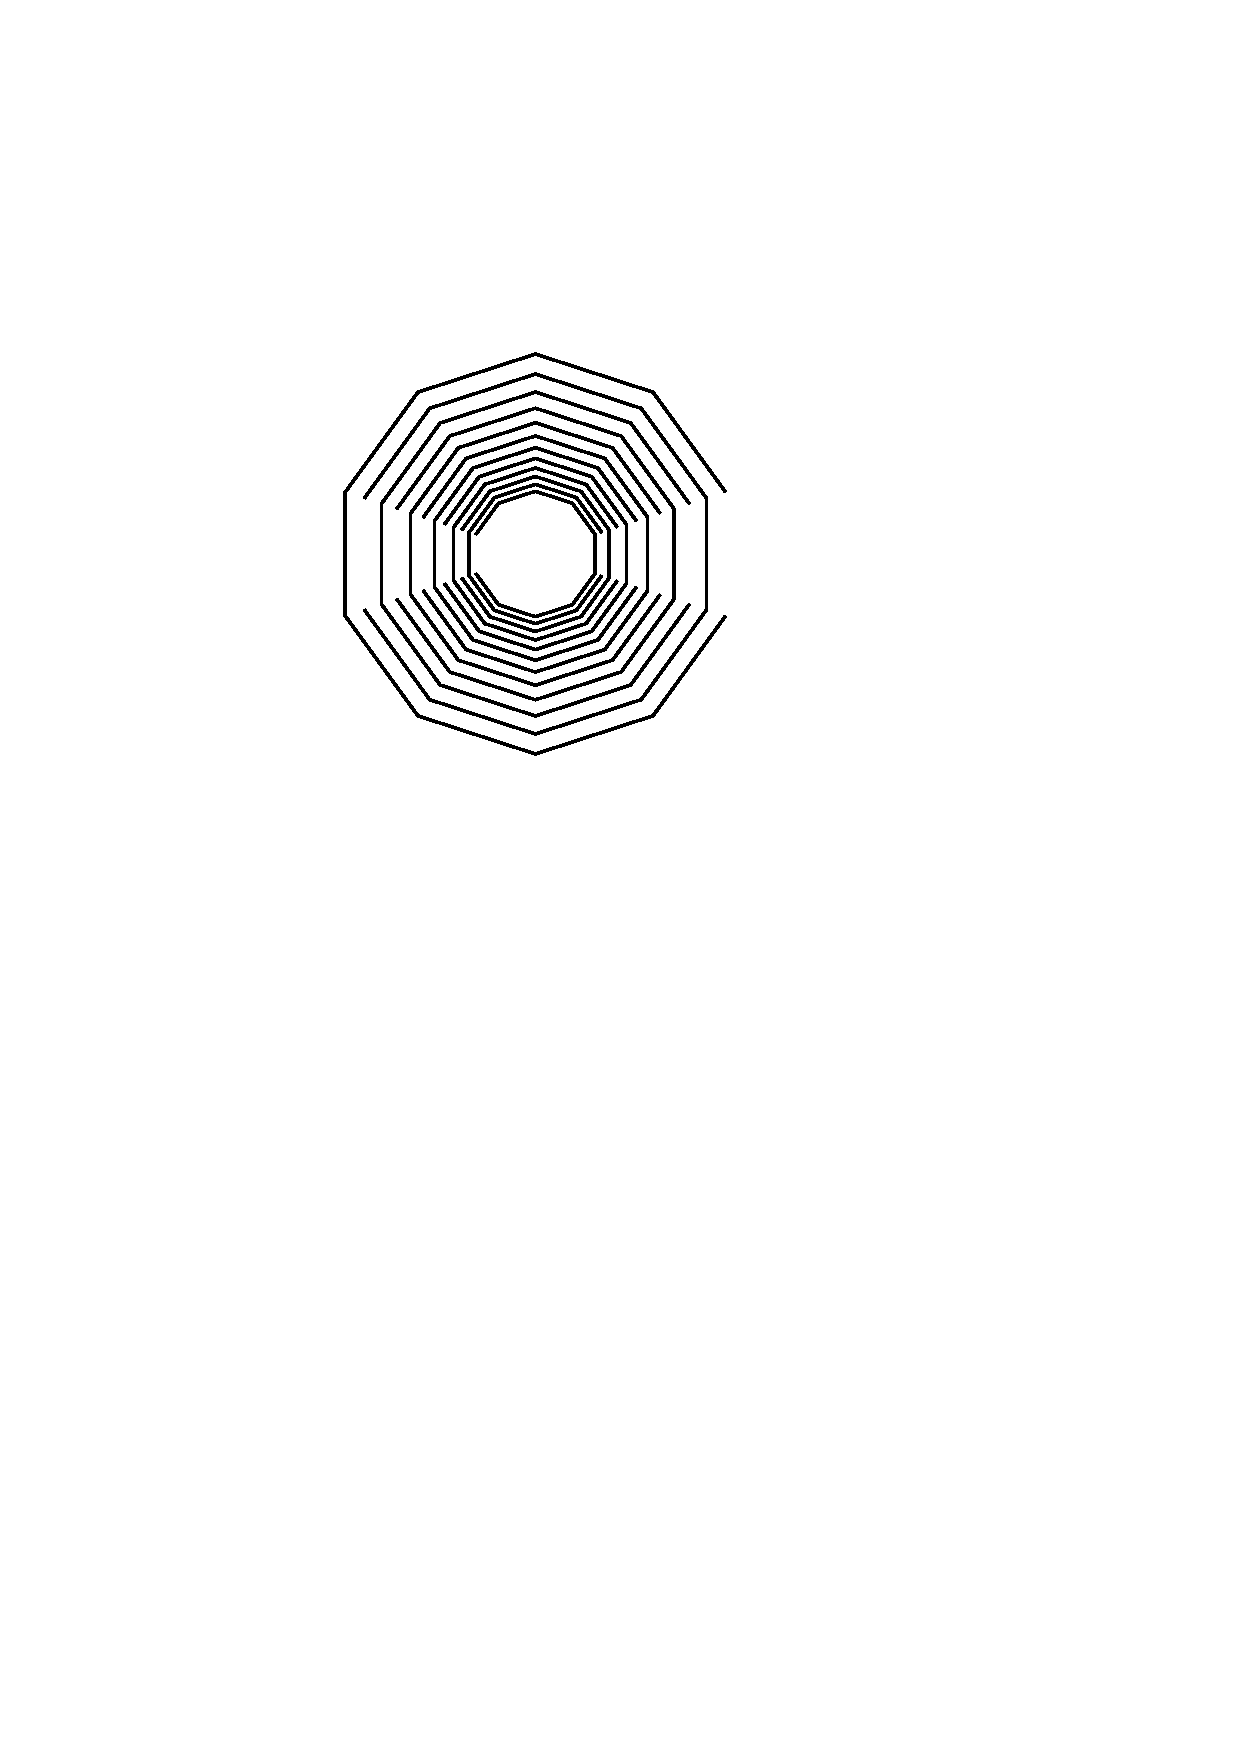
\includegraphics{lower-bound} & \includegraphics{lower-bound-b} \\
      (a) &\hspace{1cm} (b) 
      \end{tabular}
    \end{center}
    \caption{The lower-bound (a)~point set for \thmref{lower-bound}, and
      (b)~the best-case ratio $\|uw\|_G/\|uw\|$ for a pair $(u,w)$ that
      is not covered by any edge.}
    \figlabel{lower-bound}
  \end{figure}

  Let $G$ be any graph with vertex set $V$.  We say that edge a $uw$
  with $u\in A$ and $w\in B$ \emph{covers} the set of pairs
  \[
     \{ \left(u+(0,i), w+(n,j)\right) : 
          i,j\in\{-\sqrt{\alpha n},\ldots,\sqrt{\alpha n}\}\}
  \]
  for some constant $\alpha$ to be discussed later.  Thus, any edge of
  $G$ covers at most $4\alpha n$ pairs in $A\times B$.

  Next, observe that if some pair of points $u\in A$ and $w\in B$ is
  not covered by any edge of $G$, then a straightforward minimization
  argument shows that
  \[
     \frac{\|uw\|_G}{\|uw\|}
       \ge \frac{\sqrt{\alpha n}+\sqrt{(n/2)^2+(n/2-\sqrt{\alpha n})^2}}
               {n/\sqrt{2}}
       \ge \frac{\sqrt{\alpha n}+n/\sqrt{2}-O(n^{1/4})}
               {n/\sqrt{2}}
       \ge 1+\Omega(1/\sqrt{n})
  \]
  (see \figref{lower-bound}.b).
  If $G$ has $m\in O(n)$ edges, then we select $\alpha \le
  \binom{n}{2}/(8mn)$ so that
  \[  
     m4\alpha n \le \frac{\binom{n}{2}}{2} 
  \]
  In this way, at least half of the $\binom{n}{2}$ pairs of points in $V$
  are not covered by any edge and therefore,
  \[
     \asf(G) \ge 1 + \binom{n}{2}^{-1}\cdot\frac{\binom{n}{2}}{2}\cdot
          \Omega(1/\sqrt{n}) = 1 + \Omega(1/\sqrt{n}) \enspace . \qedhere
  \]
\end{proof}

We remark that the proof of \thmref{lower-bound} is easily modified to
provide a tradeoff between the number of edges of $G$ and the average
spanning ratio.  In particular, if $G$ has $m\in o(n^2)$ edges, then
\[
   \asf(G) \ge 1 + \Omega(1/\sqrt{m}) \enspace .
\]


\section*{Acknowledgement}

The authors of this paper are partly funded by NSERC and CFI.

\section*{Authors}

\noindent\emph{Vida Dujmovi\'c.}
School of Mathematics and Statistics and Department of Systems and Computer Engineering, Carleton University
%, \texttt{vida@cs.mcgill.ca}

\noindent\emph{Pat Morin} and \emph{Michiel Smid.}
School of Computer Scence, Carleton University
%, \texttt{\{morin,smid\}@scs.carleton.ca}


\bibliographystyle{abbrv}
\bibliography{avgstretch}





\end{document}


